\section{Early Antecedents}

The idea that the flow of information is a part of ecosystem processes can be traced back at least one-hundred years to the work of Verdansky, Le Roy and Teilhard in the 1920s. Preceding the rise of ecosystem thinking by perhaps a decade these thinkers proposed that the human thought, ideas, and creativity--in short human cognition--would give rise to the human power over nuclear structures in atoms so that people might literally create new elements. Much like life had transformed the geosphere into the biosphere, the development of human ideas would transform the biosphere into the \textit{noosphere}: literally translated from its Greek roots, the sphere of the mind. While this particular outcome has not yet become manifest as originally conceived, since the coining of this term many ecologists and geologists have come to call the current geological epoch the \textit{anthropocene}. This is a linguistic admission that human ideas, technology, and governance of society have tangible and observable effects on the global environment, albeit through alternative but similar means. 

At approximately the same time as the appearance of the word "ecosystem" as a push back against organismic metaphors for living communities, the librarian Ranganathan famously suggested five laws of librarianship. The last of his laws is that the Library is a growing organism. This metaphor, like others so popular at this time, including most western ecologists who perceived natural ecosystems through a holistic lens as some sort of super organism, included notions of growth, evolution, a touch of diversity, and some vitality. The library is literally alive (based on a unidentifiable Sanskrit religious metaphor) \citep{ranganathan_1931}.

While these two examples may appear far-fetched and dated, the influence of these metaphors is far-reaching. Perhaps the best examples come from the development of human ecology and cultural ecology in the field of anthropology. Similar to how ecologists measured flows of energy and nutrients to assuage their lack of scientific self confindence during the quantitative revolution, anthropologists counted calories and food exchanges in small "closed" societies. Studies claimed that culturallly defined norms, rules, and rituals helped create homeostatic systems. The flow and management of information governened by cultural institutions in these systems provided the feedback loops to maintain system stability. Much like ecologists, the anthropologists were borrowing from systems theory and cybernetics to make their arguments. This kind of thinking rose in popularity through the 1960s and 1970s only to be debunked as the scale of analysis expanded. Bernard Nietschmann, a cultural anthropologist who studied coastal Miskito communities in Nicaragua, clearly showed that if the scale of analysis includes international trade pressures, the expansion of capitalism as an economic system, and other external factors, stability of these "closed" systems quickly morphs into cultural and ecological degradation \citep{nietschmannn_1973}.

\begin{figure}[!ht]
  \centering
    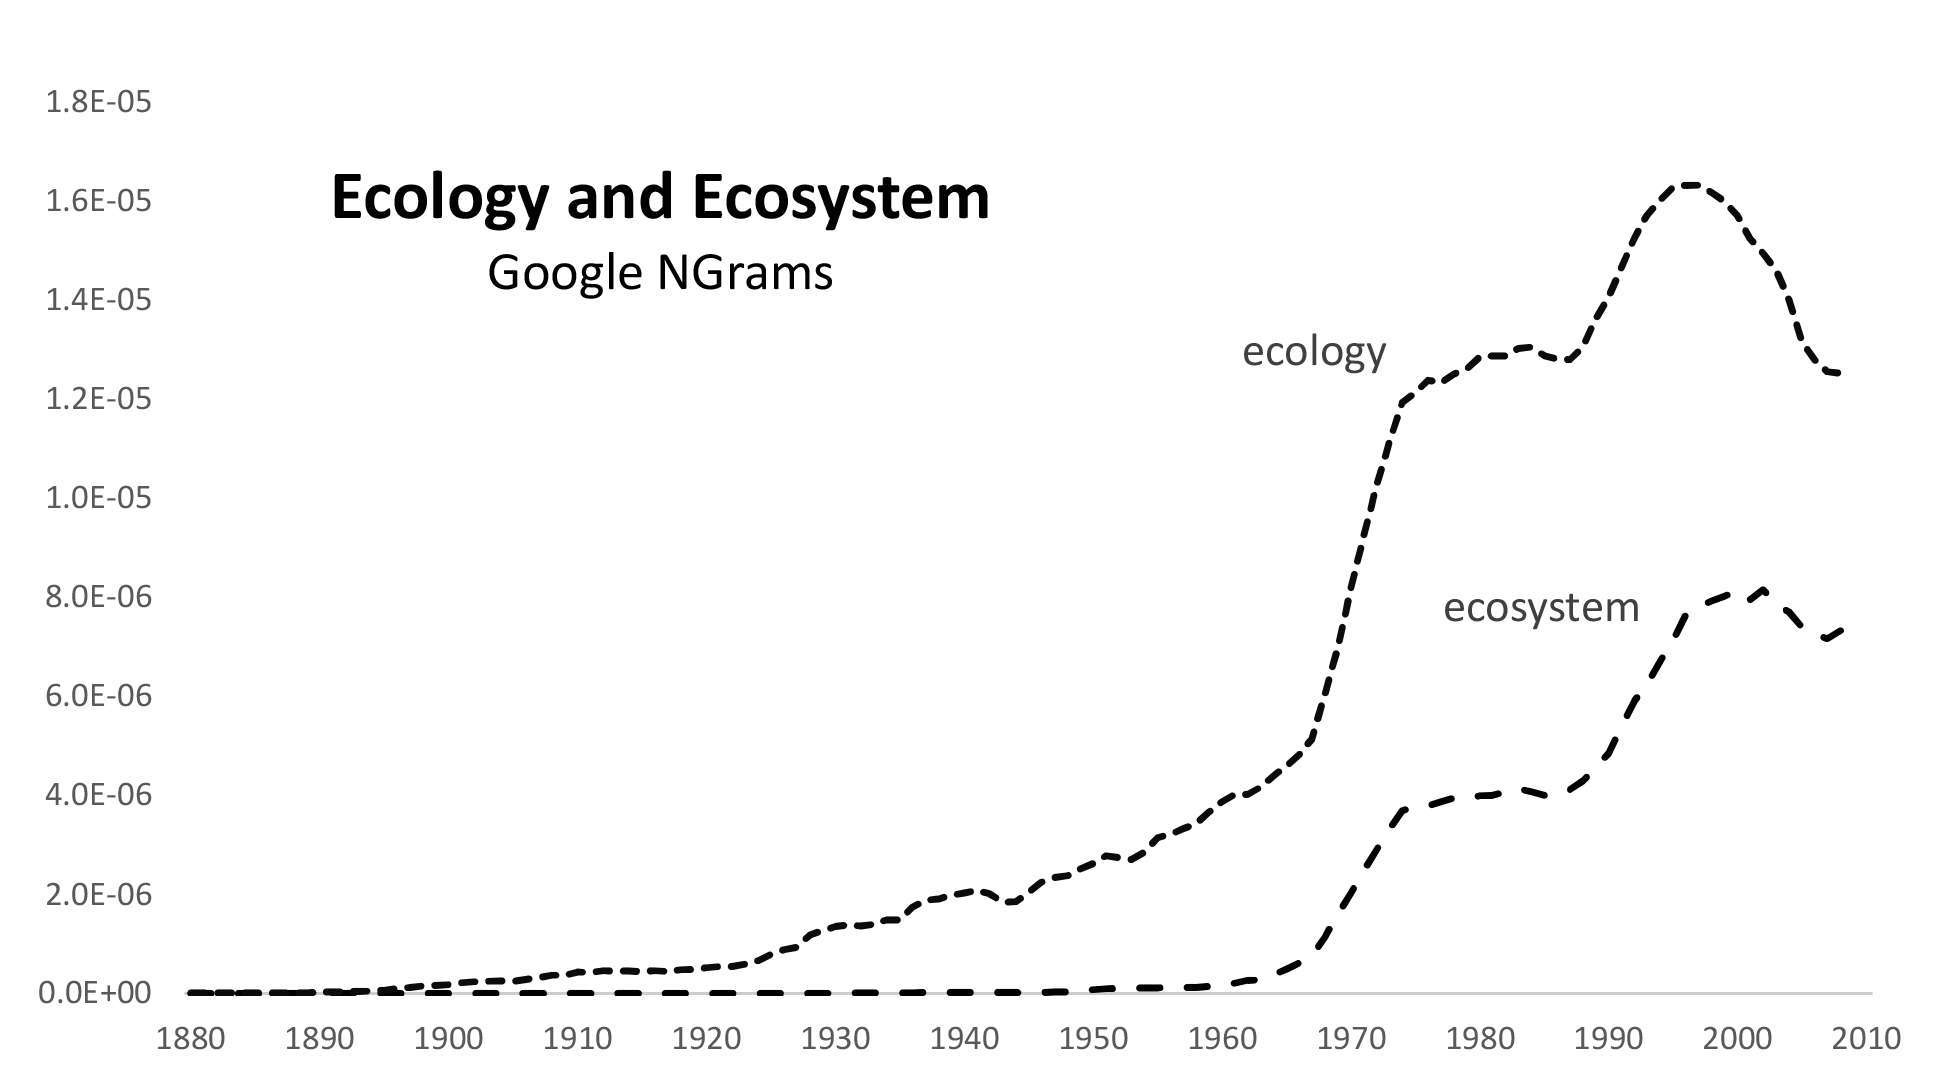
\includegraphics[width=0.9\textwidth]{figures/ecologyEcosystem}
  \caption{The rise of ecology and ecosystems.}
\end{figure} 

A common thread in these three examples is that all have a basis in the management of some kind of resource; Verdansky's noosphere in elemental resources, Ranganathan's living library in information resources, and Nietschmann's socio-ecological environments in turtles as biological resources. This emphasis on resource management was picked up in business management literature and emerged as the management of the information ecosystem, or information ecology. Yet to find a coherent program for information ecology before the publication of Nardi and O'Day's \textit{Information Ecologies} and Davenport's \textit{Information Ecology} is challenging \citep{nardi_information_1999, davenport_information_1997}. When the term was used it appeared in disconnected places. Horton Forest is perhaps the first author to use the term "information ecology" in an article title in his 1978 publication on computer systems management \citep{forest_1978} [I have this on request, hopefully get it soon, see the bib from Eryomin]. Nelson's 1985 book titled \textit{An Evolutionary Theory of Economic Change} suggested biological analogies in economic theory \citep{nelson_evolutionary_1985}. This work was later used as a base for some of the metaphors in Davenport's work [need to check this in his bib]. Kevin Harris provides one of the clearest early examples from the business management literature where the actual phrase "Information Ecology" appears. His short article titled "Information Ecology" called upon researchers to recognize the dynamic interdependence of information systems within an organization, especially businesses. According to him, organizations have a state of informedness shaped by the exchange of information from both inside and outside of an organization. He analogizes this interaction between systems within an organization as a type of ecosystem in the sense that they are self-regulating, progressive, and maintain states of dynamic equilibrium. Interestingly, he likens the goals of information managers to maintain "dynamic but stable" systems to the processes found in naturally occurring ecosystems, he even states that moderate levels of "disturbance" may be healthy in an information ecosystem. His authority for these claims is a 1968 study in the social sciences that draws the same conclusion: social systems maintain dynamic equilibriums much like those found in naturally occurring ecosystems. [He also has a background as a fellow with the British Library and at the time of writing his article was mangeing databases for a tech firm in London.] In any case the discussion is brief and not elaborated in any detail, but it is suggested that it may be a "useful analogy" \citep{harris_information_1989}.

Another interesting precursor use of the phrase "information ecologies" comes from the environmental studies literature. Eryomin adduces the importance of information to the study and understanding of the environment. Information influences the formation of biosystems, the health of human beings, and our social well-being. All of these depend upon systems for valuing, storing, transmitting, and receiving information, be it digital or analog. A program for the study of information ecology would examine each of these processes, in addition to examining the criteria for information and the communities and organizations through which it flows [this must be linked to the older versions of human ecology from which the original information ecology emerged (as far as I can tell)]. For Eryomin, information ecology has the potential to be a grand synthesis between the biological sciences and the human condition through the careful study of information exchange \citep{eryomin_information_1998}. Indeed this has again been picked up very recently as an extension of the adaptive management (AM) and Panarchy literatures \citep{eddy_information_2014}. [NOTE: I think this is an interesting late development that could be included as both a call for more research in this direction in both the conclusion and the end of the "theory" section]